\documentclass[]{article}
\usepackage{lmodern}
\usepackage{amssymb,amsmath}
\usepackage{ifxetex,ifluatex}
\usepackage{fixltx2e} % provides \textsubscript
\ifnum 0\ifxetex 1\fi\ifluatex 1\fi=0 % if pdftex
  \usepackage[T1]{fontenc}
  \usepackage[utf8]{inputenc}
\else % if luatex or xelatex
  \ifxetex
    \usepackage{mathspec}
  \else
    \usepackage{fontspec}
  \fi
  \defaultfontfeatures{Ligatures=TeX,Scale=MatchLowercase}
\fi
% use upquote if available, for straight quotes in verbatim environments
\IfFileExists{upquote.sty}{\usepackage{upquote}}{}
% use microtype if available
\IfFileExists{microtype.sty}{%
\usepackage[]{microtype}
\UseMicrotypeSet[protrusion]{basicmath} % disable protrusion for tt fonts
}{}
\PassOptionsToPackage{hyphens}{url} % url is loaded by hyperref
\usepackage[unicode=true]{hyperref}
\hypersetup{
            pdftitle={Change Point Regression},
            pdfborder={0 0 0},
            breaklinks=true}
\urlstyle{same}  % don't use monospace font for urls
\usepackage[margin=1in]{geometry}
\usepackage{color}
\usepackage{fancyvrb}
\newcommand{\VerbBar}{|}
\newcommand{\VERB}{\Verb[commandchars=\\\{\}]}
\DefineVerbatimEnvironment{Highlighting}{Verbatim}{commandchars=\\\{\}}
% Add ',fontsize=\small' for more characters per line
\usepackage{framed}
\definecolor{shadecolor}{RGB}{248,248,248}
\newenvironment{Shaded}{\begin{snugshade}}{\end{snugshade}}
\newcommand{\KeywordTok}[1]{\textcolor[rgb]{0.13,0.29,0.53}{\textbf{#1}}}
\newcommand{\DataTypeTok}[1]{\textcolor[rgb]{0.13,0.29,0.53}{#1}}
\newcommand{\DecValTok}[1]{\textcolor[rgb]{0.00,0.00,0.81}{#1}}
\newcommand{\BaseNTok}[1]{\textcolor[rgb]{0.00,0.00,0.81}{#1}}
\newcommand{\FloatTok}[1]{\textcolor[rgb]{0.00,0.00,0.81}{#1}}
\newcommand{\ConstantTok}[1]{\textcolor[rgb]{0.00,0.00,0.00}{#1}}
\newcommand{\CharTok}[1]{\textcolor[rgb]{0.31,0.60,0.02}{#1}}
\newcommand{\SpecialCharTok}[1]{\textcolor[rgb]{0.00,0.00,0.00}{#1}}
\newcommand{\StringTok}[1]{\textcolor[rgb]{0.31,0.60,0.02}{#1}}
\newcommand{\VerbatimStringTok}[1]{\textcolor[rgb]{0.31,0.60,0.02}{#1}}
\newcommand{\SpecialStringTok}[1]{\textcolor[rgb]{0.31,0.60,0.02}{#1}}
\newcommand{\ImportTok}[1]{#1}
\newcommand{\CommentTok}[1]{\textcolor[rgb]{0.56,0.35,0.01}{\textit{#1}}}
\newcommand{\DocumentationTok}[1]{\textcolor[rgb]{0.56,0.35,0.01}{\textbf{\textit{#1}}}}
\newcommand{\AnnotationTok}[1]{\textcolor[rgb]{0.56,0.35,0.01}{\textbf{\textit{#1}}}}
\newcommand{\CommentVarTok}[1]{\textcolor[rgb]{0.56,0.35,0.01}{\textbf{\textit{#1}}}}
\newcommand{\OtherTok}[1]{\textcolor[rgb]{0.56,0.35,0.01}{#1}}
\newcommand{\FunctionTok}[1]{\textcolor[rgb]{0.00,0.00,0.00}{#1}}
\newcommand{\VariableTok}[1]{\textcolor[rgb]{0.00,0.00,0.00}{#1}}
\newcommand{\ControlFlowTok}[1]{\textcolor[rgb]{0.13,0.29,0.53}{\textbf{#1}}}
\newcommand{\OperatorTok}[1]{\textcolor[rgb]{0.81,0.36,0.00}{\textbf{#1}}}
\newcommand{\BuiltInTok}[1]{#1}
\newcommand{\ExtensionTok}[1]{#1}
\newcommand{\PreprocessorTok}[1]{\textcolor[rgb]{0.56,0.35,0.01}{\textit{#1}}}
\newcommand{\AttributeTok}[1]{\textcolor[rgb]{0.77,0.63,0.00}{#1}}
\newcommand{\RegionMarkerTok}[1]{#1}
\newcommand{\InformationTok}[1]{\textcolor[rgb]{0.56,0.35,0.01}{\textbf{\textit{#1}}}}
\newcommand{\WarningTok}[1]{\textcolor[rgb]{0.56,0.35,0.01}{\textbf{\textit{#1}}}}
\newcommand{\AlertTok}[1]{\textcolor[rgb]{0.94,0.16,0.16}{#1}}
\newcommand{\ErrorTok}[1]{\textcolor[rgb]{0.64,0.00,0.00}{\textbf{#1}}}
\newcommand{\NormalTok}[1]{#1}
\usepackage{graphicx,grffile}
\makeatletter
\def\maxwidth{\ifdim\Gin@nat@width>\linewidth\linewidth\else\Gin@nat@width\fi}
\def\maxheight{\ifdim\Gin@nat@height>\textheight\textheight\else\Gin@nat@height\fi}
\makeatother
% Scale images if necessary, so that they will not overflow the page
% margins by default, and it is still possible to overwrite the defaults
% using explicit options in \includegraphics[width, height, ...]{}
\setkeys{Gin}{width=\maxwidth,height=\maxheight,keepaspectratio}
\IfFileExists{parskip.sty}{%
\usepackage{parskip}
}{% else
\setlength{\parindent}{0pt}
\setlength{\parskip}{6pt plus 2pt minus 1pt}
}
\setlength{\emergencystretch}{3em}  % prevent overfull lines
\providecommand{\tightlist}{%
  \setlength{\itemsep}{0pt}\setlength{\parskip}{0pt}}
\setcounter{secnumdepth}{0}
% Redefines (sub)paragraphs to behave more like sections
\ifx\paragraph\undefined\else
\let\oldparagraph\paragraph
\renewcommand{\paragraph}[1]{\oldparagraph{#1}\mbox{}}
\fi
\ifx\subparagraph\undefined\else
\let\oldsubparagraph\subparagraph
\renewcommand{\subparagraph}[1]{\oldsubparagraph{#1}\mbox{}}
\fi

% set default figure placement to htbp
\makeatletter
\def\fps@figure{htbp}
\makeatother

\usepackage{graphics}
\usepackage{etoolbox}
\makeatletter
\providecommand{\subtitle}[1]{% add subtitle to \maketitle
  \apptocmd{\@title}{\par {\large #1 \par}}{}{}
}
\makeatother

\title{Change Point Regression}
\author{}
\date{\vspace{-2.5em}2021-07-15}

\begin{document}
\maketitle

.column-left\{ float: left; width: 56\%; text-align: left;

\}

\emph{This implementation of change point regression was developed by
\href{https://www.plymouth.ac.uk/staff/julian-stander}{Julian Stander
(University of Plymouth)} and first published in
\href{https://www.nature.com/articles/s41561-019-0392-9}{Eichenseer et
al. (2019)}.}

Assume we want to investigate the relationship between two variables,
\(x\) and \(y\), that we have collected over a certain period of time.
We have reason to believe that the relationship changed at some point,
but we don't know when.

Let's generate \(x\) and \(y\) and plot them. \(y\) is linearly
dependent on \(x\) across the whole time series, but we induce an
increase in the intercept, slope and residual variance at the
\(35^{th}\) observation:

\begin{Shaded}
\begin{Highlighting}[]
\KeywordTok{set.seed}\NormalTok{(}\DecValTok{10}\NormalTok{) }\CommentTok{# change the seed for a different sequence of random numbers}
\NormalTok{n <-}\StringTok{ }\DecValTok{60} \CommentTok{# number of total data points}
\NormalTok{n_shift <-}\StringTok{ }\DecValTok{35} \CommentTok{# the data point at which we introduce a change}
\NormalTok{x <-}\StringTok{ }\KeywordTok{rnorm}\NormalTok{(n,}\DecValTok{0}\NormalTok{,}\DecValTok{1}\NormalTok{) }\CommentTok{# generate x}
\NormalTok{y <-}\StringTok{ }\KeywordTok{rnorm}\NormalTok{(n,}\DecValTok{0}\NormalTok{,}\FloatTok{0.5}\NormalTok{) }\OperatorTok{+}\StringTok{ }\FloatTok{0.5} \OperatorTok{*}\StringTok{ }\NormalTok{x }\CommentTok{# generate y without a change}
\NormalTok{y[n_shift}\OperatorTok{:}\NormalTok{n] <-}\StringTok{ }\KeywordTok{rnorm}\NormalTok{(}\KeywordTok{length}\NormalTok{(n_shift}\OperatorTok{:}\NormalTok{n),}\DecValTok{0}\NormalTok{,}\DecValTok{1}\NormalTok{) }\OperatorTok{+}\StringTok{ }\DecValTok{1} \OperatorTok{*}\StringTok{ }\NormalTok{x[n_shift}\OperatorTok{:}\NormalTok{n] }\OperatorTok{+}\StringTok{ }\FloatTok{0.75} \CommentTok{# introduce change}
\end{Highlighting}
\end{Shaded}

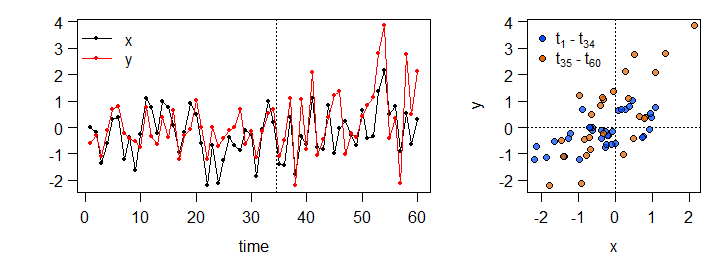
\includegraphics{index_files/figure-latex/unnamed-chunk-2-1.pdf}

\subsection{The regression model}\label{the-regression-model}

Now we build a model that can recover the change point and the linear
relationship between \(x\) and \(y\) before and after the change point.

The first part of this model looks like an ordinary least squares
regression of \(y\) against \(x\):

\(\begin{aligned} \begin{equation} \begin{array}{l} y_i \sim N(\mu_i, \sigma_1^2), ~~\\ \mu_i = \alpha_1~+~\beta_1~x_i, ~~~~~ i = 1,...,n_{change}-1 \end{array} \end{equation} \end{aligned}\)

Here we have a single intercept (\(\alpha_1\)), slope (\(\beta_1\)), and
residual variance (\(\sigma^2_1\)). \(n_{change}\) - 1 denotes the
number of obervations before the change point.

From the change point \(n_{change}\) onwards, we add an additional
intercept, \(\alpha_2\), to the intercept from the first part
(\(\alpha_1\)). We do the same for the slope and the residual variance:

\(\begin{aligned} \begin{equation} \begin{array}{l} y_i \sim N(\mu_i, \sigma_1^2+\sigma_2^2), ~~\\ \mu_i = \alpha_1~+~\alpha_2~+~(\beta_1~+~\beta_2)~x_i, ~~~~~ i = n_{change},...,n \end{array} \end{equation} \end{aligned}\)

\(n\) denotes the total number of observations, 60 in this case. But how
do we actually find the change point \(n_{change}\)?

\subsection{Implementation in JAGS}\label{implementation-in-jags}

Here, we turn to the \href{https://mcmc-jags.sourceforge.io/}{JAGS
programming environment}. Understanding a model written for JAGS is not
easy at first. If you are keen on learning Bayesian modeling from
scratch I can highly recommend Richard McElreath's book
\href{https://xcelab.net/rm/statistical-rethinking/}{Statistical
Rethinking}. We will access JAGS with the
\href{https://CRAN.R-project.org/package=R2jags}{R2jags package}, so we
can keep using R even if we are writing a model for JAGS.

Below, we look at the model. The R code that will be passed to JAGS
later is on the left. On the right is an explanation for each line of
the model.

\begin{Shaded}
\begin{Highlighting}[]
\NormalTok{model_CPR <-}\StringTok{ }\ControlFlowTok{function}\NormalTok{()\{}
  
\NormalTok{  ### Likelihood or data model part}
  \ControlFlowTok{for}\NormalTok{(i }\ControlFlowTok{in} \DecValTok{1}\OperatorTok{:}\NormalTok{n)\{}
    
\NormalTok{  y[i] }\OperatorTok{~}\StringTok{ }\KeywordTok{dnorm}\NormalTok{(mu[i], tau[i]) }

    
    
\NormalTok{  mu[i] <-}\StringTok{ }\NormalTok{alpha_}\DecValTok{1} \OperatorTok{+}\StringTok{ }
\StringTok{  }\NormalTok{alpha_}\DecValTok{2} \OperatorTok{*}\StringTok{ }\KeywordTok{step}\NormalTok{(i }\OperatorTok{-}\StringTok{ }\NormalTok{n_change) }\OperatorTok{+}
\StringTok{  }\NormalTok{(beta_}\DecValTok{1} \OperatorTok{+}\StringTok{ }\NormalTok{beta_}\DecValTok{2} \OperatorTok{*}\StringTok{ }\KeywordTok{step}\NormalTok{(i }\OperatorTok{-}\StringTok{ }\NormalTok{n_change))}\OperatorTok{*}\NormalTok{x[i]}
  
  
  
\NormalTok{  tau[i] <-}\StringTok{ }\KeywordTok{exp}\NormalTok{(log_tau[i])}
  
\NormalTok{  log_tau[i] <-}\StringTok{ }\NormalTok{log_tau_}\DecValTok{1} \OperatorTok{+}\StringTok{ }\NormalTok{log_tau_}\DecValTok{2} \OperatorTok{*}\StringTok{ }
\StringTok{  }\KeywordTok{step}\NormalTok{(i }\OperatorTok{-}\StringTok{ }\NormalTok{n_change)}
  
\NormalTok{  \} }
  
\NormalTok{  ### Priors}
  
  
\NormalTok{  alpha_}\DecValTok{1} \OperatorTok{~}\StringTok{ }\KeywordTok{dnorm}\NormalTok{(}\DecValTok{0}\NormalTok{, }\FloatTok{1.0E-4}\NormalTok{)}
  
  
\NormalTok{  alpha_}\DecValTok{2} \OperatorTok{~}\StringTok{ }\KeywordTok{dnorm}\NormalTok{(}\DecValTok{0}\NormalTok{, }\FloatTok{1.0E-4}\NormalTok{)}
  
\NormalTok{  beta_}\DecValTok{1} \OperatorTok{~}\StringTok{ }\KeywordTok{dnorm}\NormalTok{(}\DecValTok{0}\NormalTok{, }\FloatTok{1.0E-4}\NormalTok{)}
\NormalTok{  beta_}\DecValTok{2} \OperatorTok{~}\StringTok{ }\KeywordTok{dnorm}\NormalTok{(}\DecValTok{0}\NormalTok{, }\FloatTok{1.0E-4}\NormalTok{)}
  
\NormalTok{  log_tau_}\DecValTok{1} \OperatorTok{~}\StringTok{ }\KeywordTok{dnorm}\NormalTok{(}\DecValTok{0}\NormalTok{, }\FloatTok{1.0E-4}\NormalTok{)}
\NormalTok{  log_tau_}\DecValTok{2} \OperatorTok{~}\StringTok{ }\KeywordTok{dnorm}\NormalTok{(}\DecValTok{0}\NormalTok{, }\FloatTok{1.0E-4}\NormalTok{)}
  
\NormalTok{  K }\OperatorTok{~}\StringTok{ }\KeywordTok{dcat}\NormalTok{(p)}
\NormalTok{  n_change <-}\StringTok{ }\NormalTok{possible_change_points[K]}

\NormalTok{\}}
\end{Highlighting}
\end{Shaded}

We save the model as a function named \emph{model\_CPR}

Loop over all the data points \(1,...,n\)

\(y_i \sim N(\mu_i, \tau_i)\)\\
note that JAGS uses the precision \(\tau\) instead of \(\sigma^2\).
\(\tau = 1/\sigma^2\)

\emph{step} takes the value \(1\) if its argument is \(>= 0\),\\
and \(0\) otherwise, resulting in\\
\(\mu_i = \alpha_1~+~\beta_1~x_i\) ~ ~ before \(n_{change}\) and\\
\(\mu_i = \alpha_1~+~\alpha_2~+~(\beta_1~+~\beta_2)~x_i\) ~ ~ from
\(n_{change}\) ~ ~ onwards

back-transform \(log(\tau)\) to \(\tau\).

again, the \emph{step} function is used to define \(log(\tau)\) before
and after \(n_{change}\). Log-transformation is used to ensure that the
\(\tau\) resulting from \(\tau_1\) and \(\tau_2\) is positive.

We have to define priors for all parameters that are not specified by
data.

\(\alpha_1 \sim N(\mu = 0, \tau = 10^{-4})\) That is a normal
distribution with mean \(\mu = 0\) and standard deviation
\(\sigma = 100\),\\
because \(\sigma = 1/\sqrt{\tau}\)\\
\(\alpha_2 \sim N(0, 10^{-4})\)

\(\beta_1 \sim N(0, 10^{-4})\)\\
\(\beta_2 \sim N(0, 10^{-4})\)

\(log(\tau_1) \sim N(0, 10^{-4})\)\\
\(log(\tau_2) \sim N(0, 10^{-4})\)

Discrete prior on the change point. \(K\) indicates one of the possible
change points, based on the probability vector \(p\), which we need to
specify beforehand.

\\

\\
\\
\\
\\
\\
\\
\\
\\
\\
\\
\\
\\
\\
\\
\\
\\
\\
\\
\\
\\
\\
\\
\\
\\
\\
\\
\\
\\
\\
\\
\\
\\
\\
\\
\\
\\
\\
\\

Note that we put priors on \(log(\tau_1)\) and \(log(\tau_2)\), rather
than on \(\tau_1\) and \(\tau_2\) directly, to ensure that the precision
\(\tau\) in the second part of the regression always remains positive.
\(e^{log(\tau_1) + log(\tau_2)}\) is always \(> 0\), even if the term
\(log(\tau_1)\) + \(log(\tau_2)\) becomes negative.

Prepare the data which we pass to JAGS along with the model:

\begin{Shaded}
\begin{Highlighting}[]
\CommentTok{# minimum number of the data points before and after the change}
\NormalTok{  min_segment_length <-}\StringTok{ }\DecValTok{5} 

\CommentTok{# assign indices to the potential change points we allow}
\NormalTok{  possible_change_points <-}\StringTok{ }\NormalTok{(}\DecValTok{1}\OperatorTok{:}\NormalTok{n)[(min_segment_length}\OperatorTok{+}\DecValTok{1}\NormalTok{)}\OperatorTok{:}\NormalTok{(n}\OperatorTok{+}\DecValTok{1}\OperatorTok{-}\NormalTok{min_segment_length)] }
 
\CommentTok{# number of possible change points}
\NormalTok{  M <-}\StringTok{ }\KeywordTok{length}\NormalTok{(possible_change_points)  }

\CommentTok{# probabilities for the discrete uniform prior on the possible change points, }
\CommentTok{# i.e. all possible change points have the same prior probability}
\NormalTok{  p <-}\StringTok{ }\KeywordTok{rep}\NormalTok{(}\DecValTok{1} \OperatorTok{/}\StringTok{ }\NormalTok{M, }\DataTypeTok{length =}\NormalTok{ M) }
 
\CommentTok{# save the data to a list for jags}
\NormalTok{  data_CPR <-}\StringTok{ }\KeywordTok{list}\NormalTok{(}\StringTok{"x"}\NormalTok{, }\StringTok{"y"}\NormalTok{, }\StringTok{"n"}\NormalTok{, }\StringTok{"possible_change_points"}\NormalTok{, }\StringTok{"p"}\NormalTok{) }
\end{Highlighting}
\end{Shaded}

Load the \emph{R2jags} package to access \emph{JAGS} in \emph{R}:

\begin{Shaded}
\begin{Highlighting}[]
  \KeywordTok{require}\NormalTok{(R2jags) }
\end{Highlighting}
\end{Shaded}

Now we execute the change point regression. We instruct JAGS to run
three seperate chains so we can verify that the results are consistent.
We allow 2000 iterations for each chain, the first 1000 of each will
automatically be discared as burn-in.

\begin{Shaded}
\begin{Highlighting}[]
\NormalTok{ CPR  <-}\StringTok{ }\KeywordTok{jags}\NormalTok{(}\DataTypeTok{data =}\NormalTok{ data_CPR, }
                         \DataTypeTok{parameters.to.save =} \KeywordTok{c}\NormalTok{(}\StringTok{"alpha_1"}\NormalTok{, }\StringTok{"alpha_2"}\NormalTok{, }
                                                \StringTok{"beta_1"}\NormalTok{,}\StringTok{"beta_2"}\NormalTok{,}
                                                \StringTok{"log_tau_1"}\NormalTok{,}\StringTok{"log_tau_2"}\NormalTok{,}
                                                \StringTok{"n_change"}\NormalTok{), }
                         \DataTypeTok{n.iter =} \DecValTok{2000}\NormalTok{, }
                         \DataTypeTok{n.chains =} \DecValTok{3}\NormalTok{,}
                         \DataTypeTok{model.file =}\NormalTok{ model_CPR)}
\end{Highlighting}
\end{Shaded}

\subsection{The results}\label{the-results}

To visualise the results and inspect the posterior, we are using the
\emph{ggmcmc} package, which relies on the \emph{ggplot2} package. For
brevity, we just look at the \(n_{change}\) parameter here.

\begin{Shaded}
\begin{Highlighting}[]
\KeywordTok{library}\NormalTok{(ggmcmc)}
\NormalTok{CPR.ggs <-}\StringTok{ }\KeywordTok{ggs}\NormalTok{(}\KeywordTok{as.mcmc}\NormalTok{(CPR)) }\CommentTok{# convert to ggs object}
\KeywordTok{ggs_traceplot}\NormalTok{(CPR.ggs, }\DataTypeTok{family =} \StringTok{"n_change"}\NormalTok{) }
\end{Highlighting}
\end{Shaded}

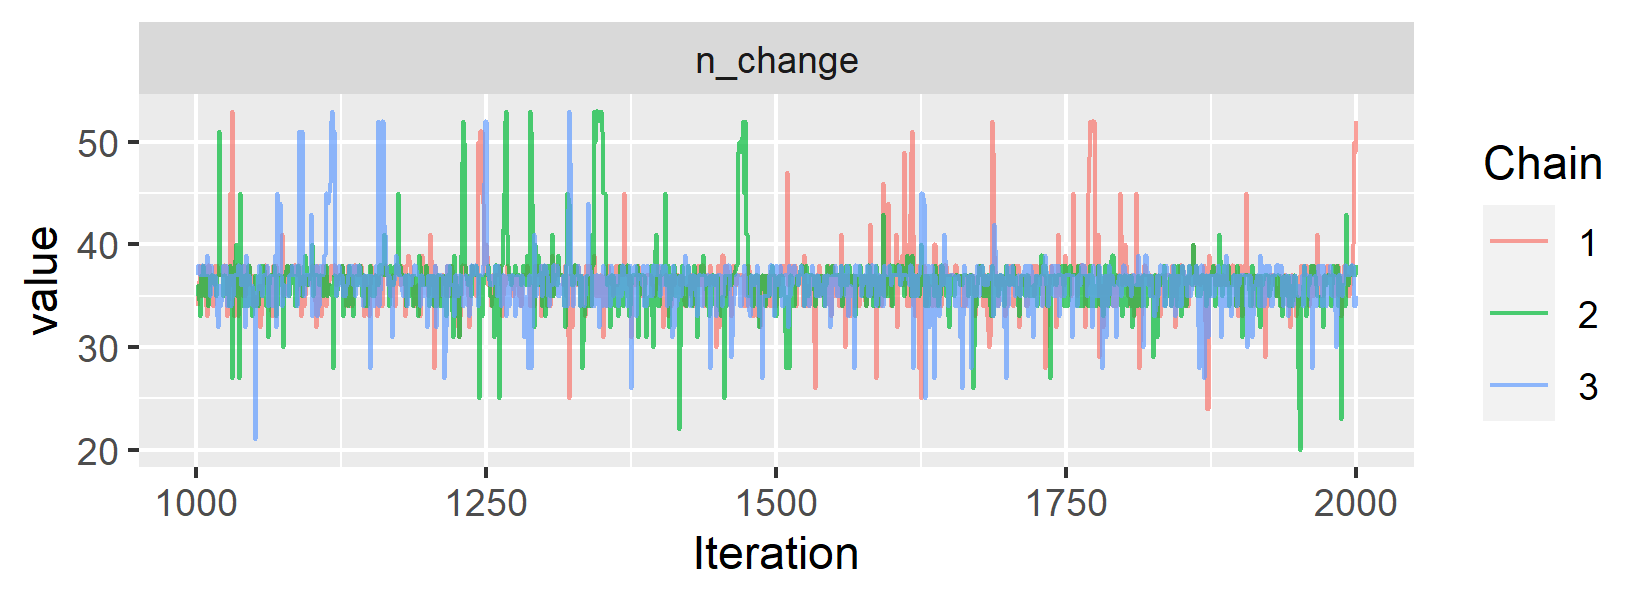
\includegraphics[width=1000 %]{index_files/figure-latex/unnamed-chunk-7-1}

Looks like the chains converge and mix nicely. We can already see that
our model locates the change point somewhere between \(30\) and \(40\),
although the chains occasionally explore regions further away.

Let's look at the posterior probabilities for the possible change
points:

\begin{Shaded}
\begin{Highlighting}[]
\KeywordTok{ggplot}\NormalTok{(}\DataTypeTok{data =}\NormalTok{ CPR.ggs }\OperatorTok\StringTok{ }\KeywordTok{filter}\NormalTok{(Parameter }\OperatorTok{==}\StringTok{ "n_change"}\NormalTok{),}
  \KeywordTok{aes}\NormalTok{(}\DataTypeTok{x=}\NormalTok{value, }\DataTypeTok{y =} \DecValTok{3}\OperatorTok{*}\NormalTok{(..count..)}\OperatorTok{/}\KeywordTok{sum}\NormalTok{(..count..), }\DataTypeTok{fill =} \KeywordTok{as.factor}\NormalTok{(Chain))) }\OperatorTok{+}\StringTok{ }
\StringTok{  }\KeywordTok{geom_vline}\NormalTok{(}\DataTypeTok{xintercept =} \DecValTok{35}\NormalTok{,}\DataTypeTok{lty =} \DecValTok{2}\NormalTok{) }\OperatorTok{+}\StringTok{ }\KeywordTok{geom_bar}\NormalTok{(}\DataTypeTok{position =} \StringTok{"identity"}\NormalTok{, }\DataTypeTok{alpha =} \FloatTok{0.5}\NormalTok{) }\OperatorTok{+}
\StringTok{  }\KeywordTok{ylab}\NormalTok{(}\StringTok{"posterior probability"}\NormalTok{) }\OperatorTok{+}\StringTok{ }\KeywordTok{xlab}\NormalTok{(}\StringTok{"n_change"}\NormalTok{) }\OperatorTok{+}\StringTok{ }\KeywordTok{labs}\NormalTok{(}\DataTypeTok{fill=}\StringTok{'Chain'}\NormalTok{)}
\end{Highlighting}
\end{Shaded}

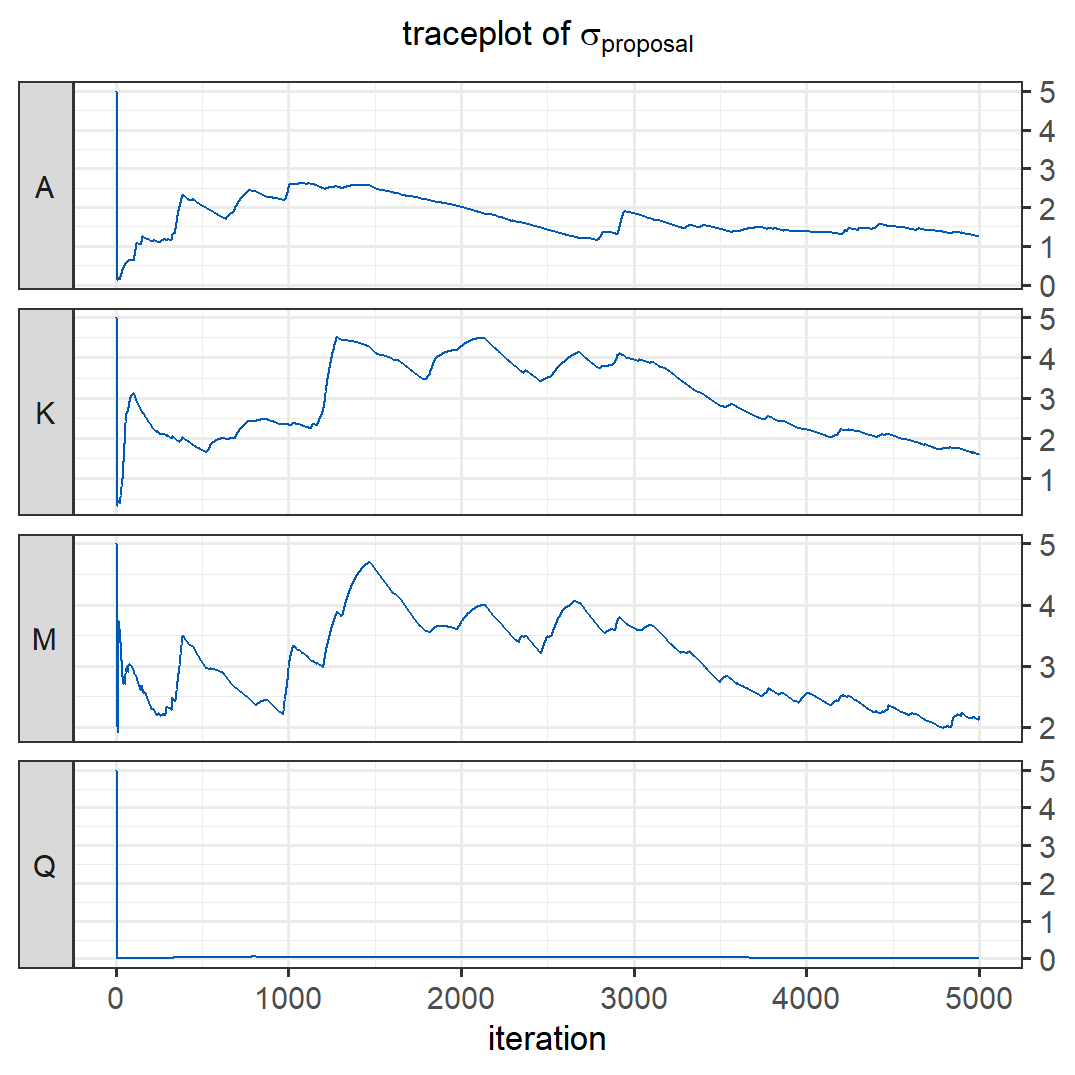
\includegraphics[width=700 %]{index_files/figure-latex/unnamed-chunk-8-1}

The \(37^{th}\) point has the highest probability of being the change
point. That is not far off from where we introduced the change, at the
\(35^{th}\) point (dashed line). The random generation of \(x\) and
\(y\) has led to \(37\) being favoured. We also note that there are only
minor differences between the three chains, and those differences would
likely further dwindle if we were to let the chains run for longer.

Using the posterior distribution, we can answer questions like: ``In
which interval does the change point fall with 90 \% probability?''

\begin{Shaded}
\begin{Highlighting}[]
\KeywordTok{quantile}\NormalTok{(CPR}\OperatorTok{$}\NormalTok{BUGSoutput}\OperatorTok{$}\NormalTok{sims.list}\OperatorTok{$}\NormalTok{n_change, }\DataTypeTok{probs =} \KeywordTok{c}\NormalTok{(}\FloatTok{0.05}\NormalTok{, }\FloatTok{0.95}\NormalTok{))}
\end{Highlighting}
\end{Shaded}

\begin{verbatim}
##  5% 95% 
##  33  39
\end{verbatim}

We can also inquire about the probability that the change point falls in
the interval \(34\) to \(38\):

\begin{Shaded}
\begin{Highlighting}[]
\KeywordTok{round}\NormalTok{(}\KeywordTok{length}\NormalTok{(}\KeywordTok{which}\NormalTok{(CPR}\OperatorTok{$}\NormalTok{BUGSoutput}\OperatorTok{$}\NormalTok{sims.list}\OperatorTok{$}\NormalTok{n_change }\OperatorTok\StringTok{ }\DecValTok{34}\OperatorTok{:}\DecValTok{38}\NormalTok{))}\OperatorTok{/}
\StringTok{              }\NormalTok{(CPR}\OperatorTok{$}\NormalTok{BUGSoutput}\OperatorTok{$}\NormalTok{n.sims),}\DecValTok{2}\NormalTok{)}
\end{Highlighting}
\end{Shaded}

\begin{verbatim}
## [1] 0.87
\end{verbatim}

Finally, let's have a look at the regression parameters and plot the
resulting regressions before and after the most likely change point.

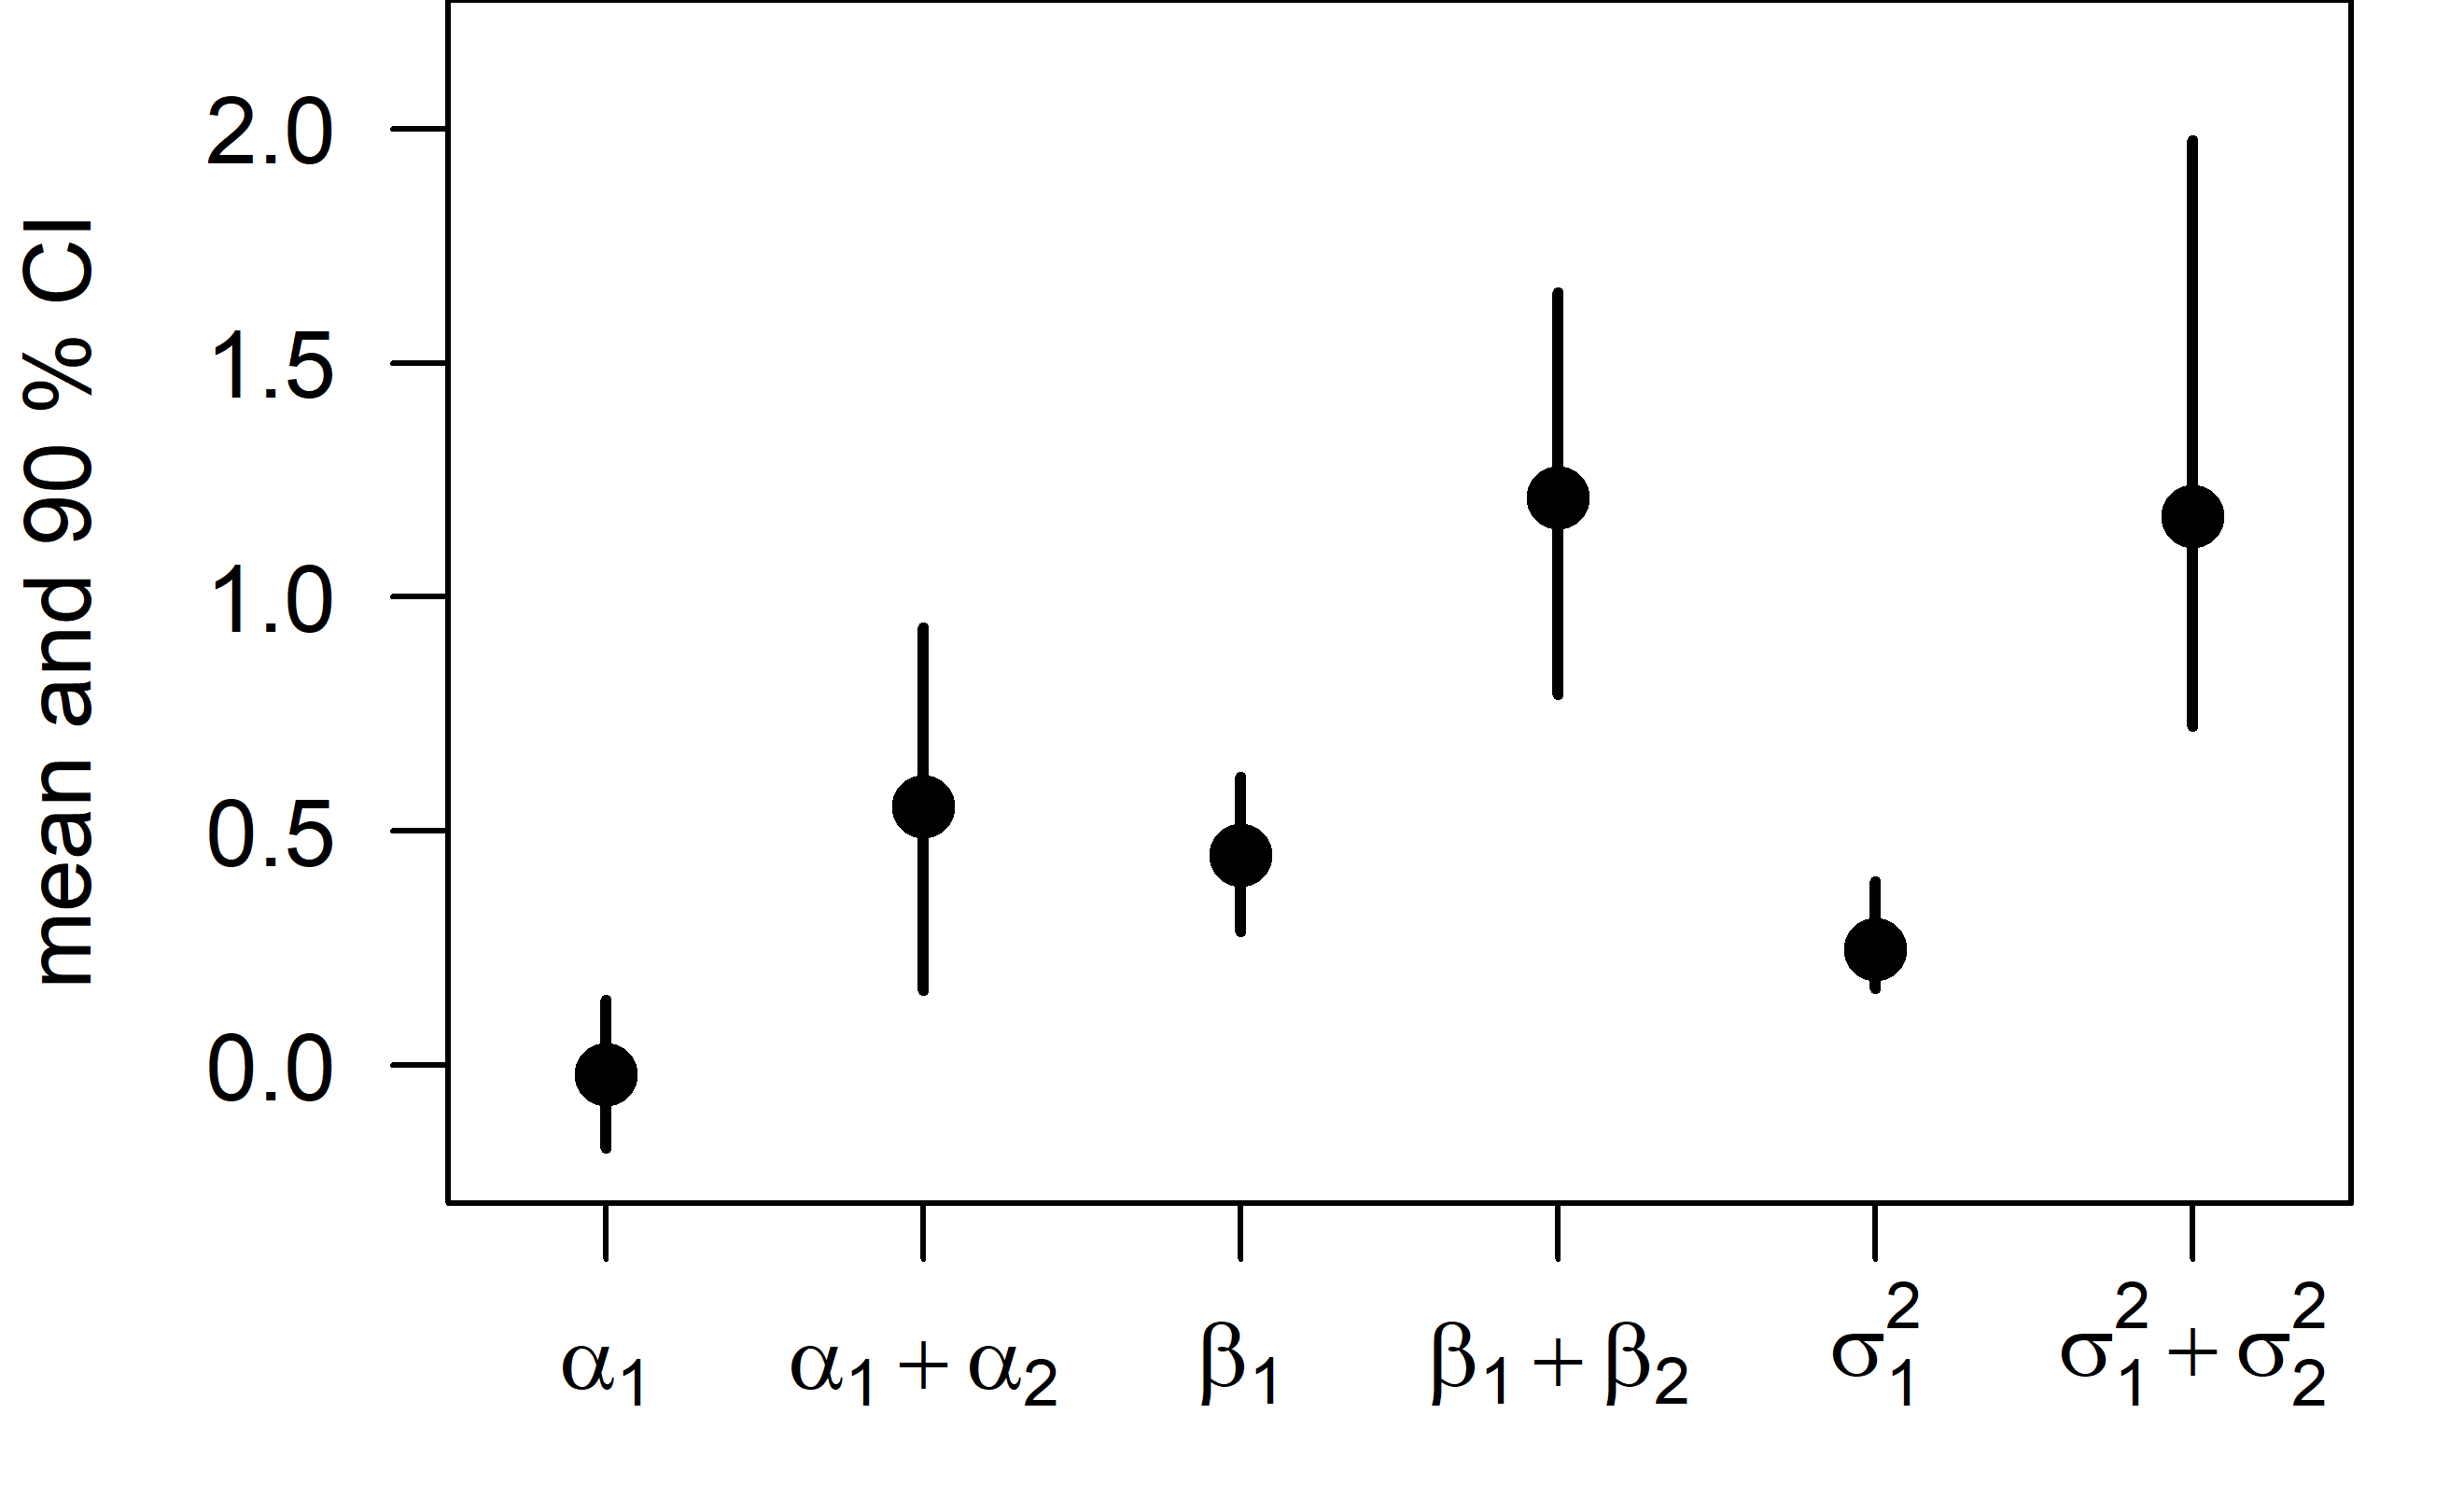
\includegraphics[width=475 %]{index_files/figure-latex/unnamed-chunk-12-1}
The intercept, slope, and residual variance all increase after the
change point.

This can be immediately seen when plotting the change point regression:

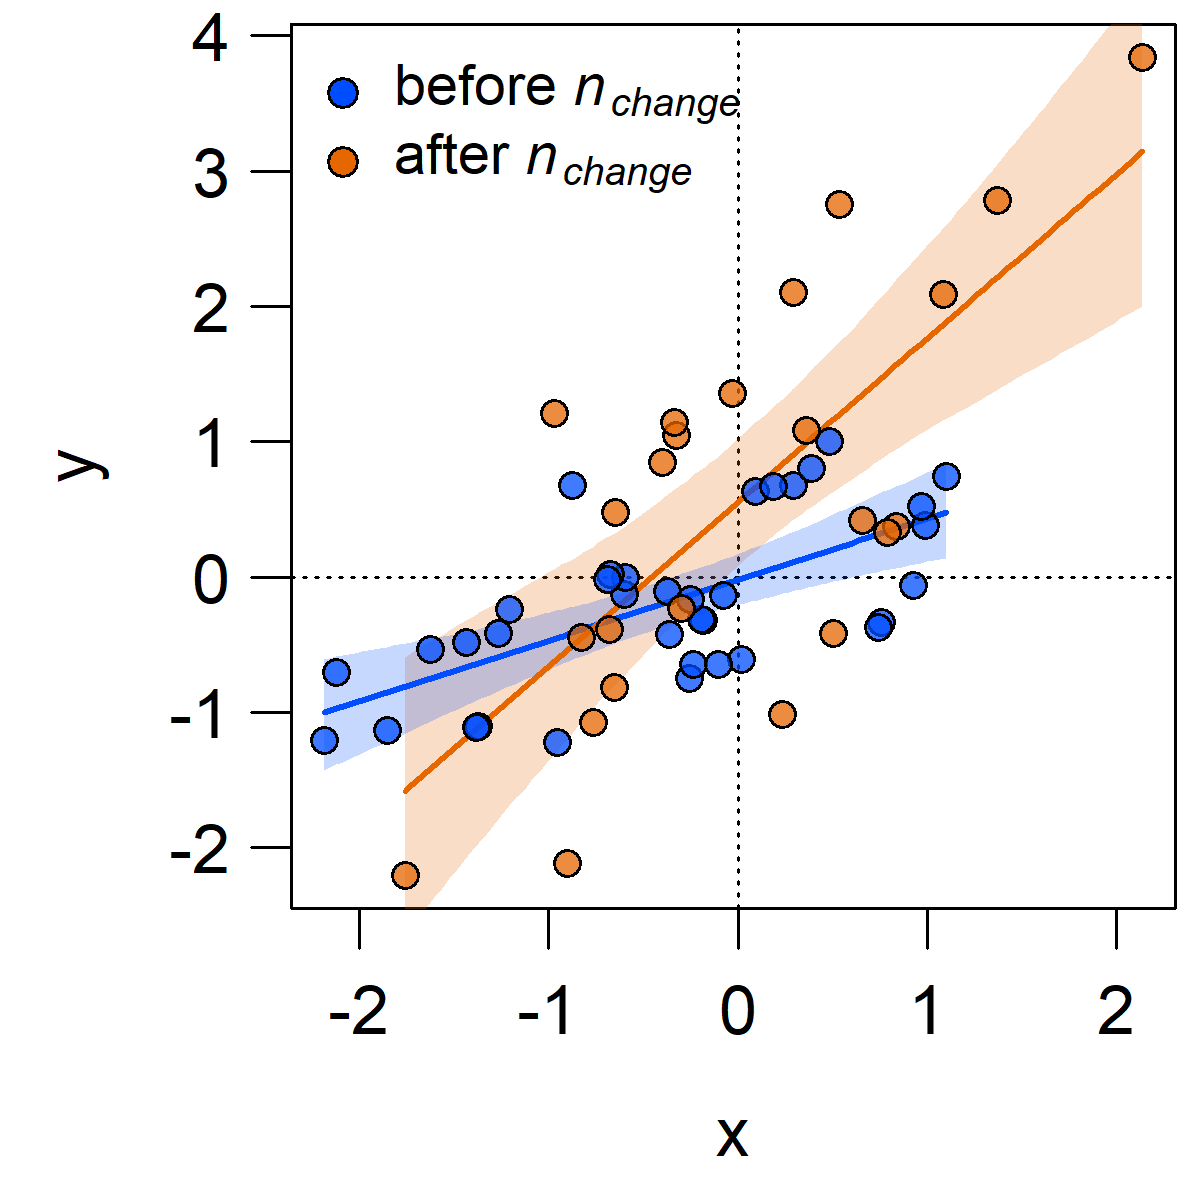
\includegraphics[width=375 %]{index_files/figure-latex/unnamed-chunk-13-1}
The shaded areas denote \(95\) \% credible intervals around the
regression lines.

You can find the full R code for this analysis at
\url{https://github.com/KEichenseer/Methods/blob/main/Change_point_regression.R}

Get in touch if you have any comments or questions!

\end{document}
